%========================================================================================%
%					NOTE
%========================================================================================%
% Probably this theme will not compile with standard pdftolatex compiler due to lack of some 
% fonts used in the theme. It is recommended to compile with XeLaTex instead.

% !TEX program = xelatex

%========================================================================================%
%					DOCUMENT SETUP
%========================================================================================%
\documentclass{beamer} 
\usetheme[progressbar=frametitle]{metropolis}

\usepackage{textpos}
\usepackage{xcolor}

\usepackage{amsmath}
\usepackage{amsfonts}
\usepackage{amssymb}

\usepackage{minted}

\usepackage{mathrsfs}
\usepackage{epstopdf}

%For making diagram and drawing
\usepackage{tikz}
\usetikzlibrary{shapes,positioning}

%For appendix
\usepackage{appendixnumberbeamer}

\usepackage[export]{adjustbox}

%Some additional graphcs tools
\usepackage{graphicx}
\graphicspath{{../figures/}{../logos/}}

%Remove words break, wrap instead
\usepackage[none]{hyphenat}


%for custom date
\usepackage[english]{babel}
\usepackage[nodayofweek,level]{datetime}

\usepackage{xspace}
\newcommand{\themename}{\textbf{\textsc{metropolis}}\xspace}

%===================================================================================%
%				FRONT PAGE
%===================================================================================%
\titlegraphic{%
\hfill%

\includegraphics[height=1.5cm, valign=c]{ccfd3.png}%
\hspace{15pt}%

\includegraphics[height=1.5cm, valign=c]{symbol-PL.pdf}%
}

\author{Jakub Gałecki}
\title{Presentation template}
\institute{Division of Aerodynamics}
\date{\vspace{5pt}\formatdate{22}{2}{2022}}

%===================================================================================%
%				THEME COLORS
%===================================================================================%
% specify main colors which are being used by the theme
\definecolor{bordercolor}{HTML}{002699}
\definecolor{fillcolor}{HTML}{002699}

% fix theme black color which affects tikz plots
\definecolor{black}{RGB}{0,0,0}

%===================================================================================%
%				ACTUAL DOCUMENT CONTENT
%===================================================================================%

\begin{document}

\maketitle

%force to add logos to the each frame title
\addtobeamertemplate{frametitle}{}{%
\begin{textblock*}{100mm}(.9\textwidth,-1cm)

\includegraphics[height=0.8cm, valign=c]{ccfd3_white.png}\hspace{10pt}
\includegraphics[height=0.78cm, valign=c]{symbol-PL-white.pdf}
\end{textblock*}}

\begin{frame}{Agenda}
\begin{itemize}
\item Item 1
\item Item 2
\item Item 3
\item Item 4
\end{itemize}
\end{frame}

\section{Section title}
\begin{frame}{Equation}
This is a regular equation 2:
\begin{equation}
\mathbf{A}\mathbf{x} = \textbf{b}
\end{equation}
And this is an equation in a block
\metroset{block=fill}
\begin{block}{Important equation}
\begin{equation}
\mathbf{C}\mathbf{y} = \textbf{d}
\end{equation}
\end{block}
\end{frame}

\begin{frame}[fragile]{Code}
\begin{minted}{c++}
#include <cstdio>
int main() {
  puts("Hello, World!");
}
\end{minted}
\end{frame}

\begin{frame}{Figures}
Vortex streets sure are pretty
\begin{figure} % you can also include the graphic directly in the frame, without the figure
\center

\includegraphics[width=0.8\textwidth]{vortex-street.jpg}
\caption{I mean look at how beautiful this this thing is!}
\end{figure}
\end{frame}

\begin{frame}{Tikz diagram}
\center
\small
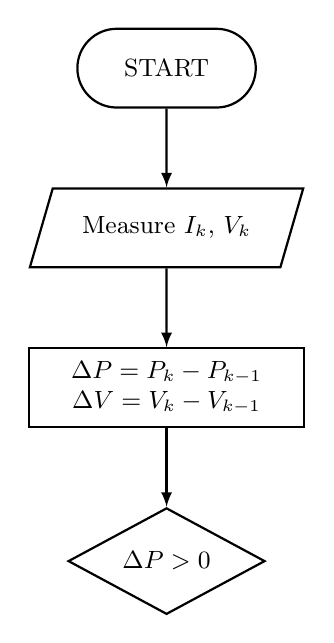
\begin{tikzpicture}[font=\small,thick]

% Start block
\node[draw,
    rounded rectangle,
    minimum width=2.5cm,
    minimum height=1cm] (block1) {START};

% Voltage and Current Measurement
\node[draw,
    trapezium, 
    trapezium left angle = 65,
    trapezium right angle = 115,
    trapezium stretches,
    below=of block1,
    minimum width=3.5cm,
    minimum height=1cm
] (block2) { Measure $I_k$, $V_k$ };

% Power and voltage variation
\node[draw,
    align=center,
    below=of block2,
    minimum width=3.5cm,
    minimum height=1cm
] (block3) { $\Delta P=P_k-P_{k-1}$ \\ $\Delta V=V_k-V_{k-1}$};

% Conditions test
\node[draw,
    diamond,
    below=of block3,
    minimum width=2.5cm,
    inner sep=0] (block4) { $\Delta P>0$};

% Arrows
\draw[-latex] (block1) edge (block2)
    (block2) edge (block3)
    (block3) edge (block4);

\end{tikzpicture}
\end{frame}

\begin{frame}[standout]
Possible transition slide
\end{frame}
\appendix
\begin{frame}{Appendix slide}
Slides in the appendix don't count towards to the progress bar
\end{frame}
\end{document}